% Initialisation
\documentclass[english,12pt]{scrartcl}

\usepackage[]{babel}
% Input is utf8
\usepackage[utf8]{inputenc}
% Enables headers and footers
\usepackage[]{scrpage2}
% Lets us colour table cells
\usepackage[table]{xcolor}
% Allows todo list and todos
\usepackage[]{todonotes}
% Makes links in contents hyperlinked
\usepackage{hyperref}
% Make references appear in our table of contents
\usepackage[nottoc,numbib]{tocbibind}
% Allows us to put landscape sections of the document
\usepackage{lscape} % \usepackage{lscape} %Use escape for printing (doesn't rotate the pdf page)
% Provides a glossary
\usepackage[toc]{glossaries}

% Gives us pretty diagrams
\usepackage{tikz}
\usetikzlibrary{calc,fit,positioning,chains,decorations.pathreplacing,shapes,backgrounds}

% Document Title and Author
\title{
\includegraphics[width=0.75\textwidth]{./Logo/NUClear-logo}~\\[1cm] NU-Architecture Requirements Document}
\author{2013 Final Year Project}

% Header and Footer
\pagestyle{scrheadings}
\ihead{\today}
\chead{}
\ohead{NU-Architecture Requirements Document}
\ifoot{}
\cfoot{}
\ofoot{\pagemark}

% Requirements custom commands
\newcommand{\requirement}[1]{\textit{#1}}

% tikz custom shapes
\tikzset{
	old inner xsep/.estore in=\oldinnerxsep,
	old inner ysep/.estore in=\oldinnerysep,
	double circle/.style 2 args={
		circle,
		old inner xsep=\pgfkeysvalueof{/pgf/inner xsep},
		old inner ysep=\pgfkeysvalueof{/pgf/inner ysep},
		/pgf/inner xsep=\oldinnerxsep+#1,
		/pgf/inner ysep=\oldinnerysep+#1,
		alias=sourcenode,
		append after command={
		let \p1 = (sourcenode.center),
		    \p2 = (sourcenode.east),
		    \n1 = {\x2-\x1-#1-0.5*\pgflinewidth}
		in
			node [inner sep=0pt, draw, circle, minimum width=2*\n1,at=(\p1),#2] {}
		}
	},
	double circle/.default={-3pt}{black!80},
	reactor/.style={draw,double circle},
	connection/.style={
		->,
		line width=0.2em
	},
	write/.style={
		->,
		thick
	},
	read/.style={
		<-,
		thick
	},
	readwrite/.style={
		<->,
		thick
	}
}

% Skip line rather then indent paragraphs
\setlength{\parindent}{0.0in}
\setlength{\parskip}{0.1in}

% Make our glossary
\makeglossaries

% Our glossary
\newglossaryentry{powerplant}
{
	name=Power Plant,
	description={
		is the central component of the Proposed Architecture that links all other components together
	}
}

\newglossaryentry{reactor}
{
	name=Reactor,
	description={
		is the name given to components that can send/recieve data. A reactor contains a number of \glspl{reaction}
	}
}

\newglossaryentry{reaction}
{
	name=Reaction,
	description={
		is the name given to a function that is called when new data is recieved.
	}
}

\newglossaryentry{nubots}
{
	name=NUBots,
	description={
		is the team responsible for programming and maintaining the robots.
	}
}

\newglossaryentry{robocup}
{
	name=RoboCup,
	description={
		is the robotic soccer competition held each year in which the NUbots compete
	}
}

% Start of document
\begin{document}
	\maketitle
	\vfill
	{\large
		\begin{description}
			\item [Status:] Release 1
			\item [Version:] 1.0
		\end{description}}

	\clearpage
	\tableofcontents
	\clearpage

	\section{Introduction}
		It is often important when working with software, that the developer takes a step back and evaluates the work.
		The University of Newcastle \gls{nubots} team have in previous years achieved success in the \gls{robocup} competition, placing several times.
		However, in recent years, the team has undergone a change in robotic platform from the \emph{Aldebaran Nao} to the \emph{Robotis DARwIn-OP}, as well as making continuous compromises in code quality to achieve deadlines.
		As a result, the software architecture of the current system has become a bastardised version of its original intent.
		The \gls{nubots} team, as a result of this have decided to replace the existing architecture with a new more effective architecture.

		This document outlines the existing architecture, what benefits can be gained from its replacement as well as the issues that warrant its replacement.
		Additionally, it also proposes a new architecture that is designed to address these issues as well as provide enhancements that will allow the system to perform effectively now and into the future.

		Finally, this document outlines the criteria by which this proposed architecture will be measured. The project team achieves this by providing a list of requirements that the proposed architecture must satisfy.

	\section{Overview}
		This section provides an overview of the existing architecture and the proposed architecture.

		\subsection{Existing Architecture}

			\begin{figure}
				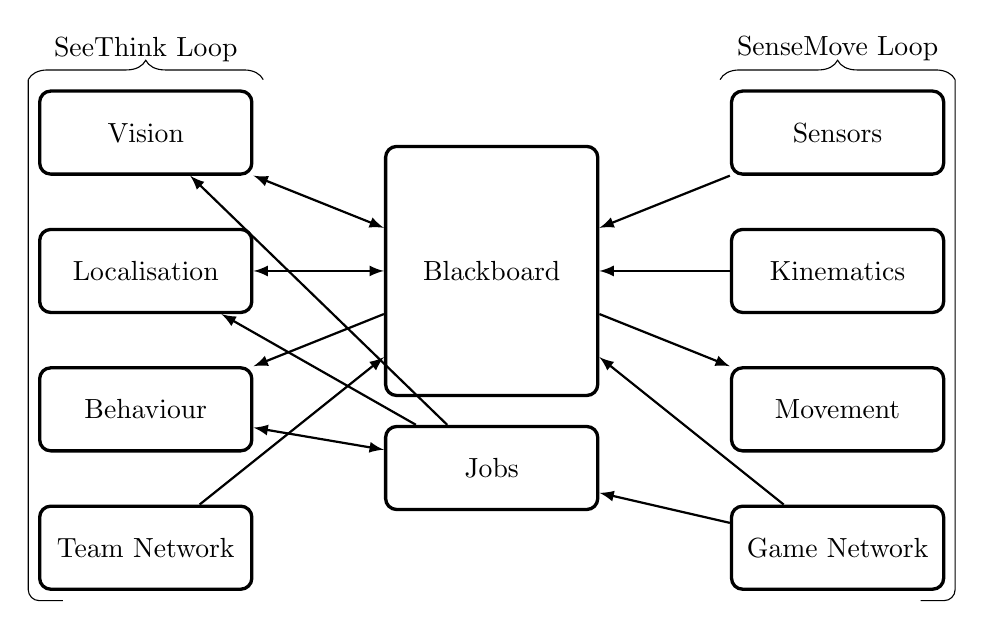
\begin{tikzpicture}[
					x=12.5em,y=5em,
					component/.style={
						rectangle,
						rounded corners,
						draw=black, very thick,
						text width=7em,
						minimum height=3em,
						text centered
					},
					>=latex]

					%%% Nodes
					%% Left hand Side
					\node at (0,3) [component] (vision) {Vision};
					\node at (0,2) [component] (localisation) {Localisation};
					\node at (0,1) [component] (behaviour) {Behaviour};
					\node at (0,0) [component] (teamnetwork) {Team Network};

					%% Center
					\node at (1, 2) [component,minimum height=9em] (blackboard) {Blackboard};
					\node [below=1em of blackboard,component] (jobs) {Jobs};

					%% Right hand side
					\node at(2,3) [component] (sensors) {Sensors};
					\node at(2,2) [component] (kinematics) {Kinematics};
					\node at(2,1) [component] (movement) {Movement};
					\node at(2,0) [component] (gamenetwork) {Game Network};

					%%% Connections
					%% Left hand blackboard connections
					\path [readwrite] (vision) edge (blackboard);
					\path [readwrite] (localisation) edge (blackboard);
					\path [read] (behaviour) edge (blackboard);
					\path [write] (teamnetwork) edge (blackboard);

					%% Left hand jobs connections
					\path [read] (vision) edge (jobs);
					\path [read] (localisation) edge (jobs);
					\path [readwrite] (behaviour) edge (jobs);

					%% Right hand blackboard connections
					\path [write] (sensors) edge (blackboard);
					\path [write] (kinematics) edge (blackboard);
					\path [read] (movement) edge (blackboard);
					\path [write] (gamenetwork) edge (blackboard);

					%% Right hand jobs connections
					\path [write] (gamenetwork) edge (jobs);

					%%% Decorations
					%% SeeThink header
					\node[fit=(vision)(localisation)(behaviour)(teamnetwork)](leftgroup){};
					\draw[rounded corners]
						(leftgroup.north west)--(leftgroup.south west) -- ++(0.10,0);
					\draw[decorate,decoration={amplitude=7pt,brace}] % Header line
						(leftgroup.north west) -- (leftgroup.north east);

					\node[above=1.1em of leftgroup,anchor=center]{SeeThink Loop};

					%% SenseMove header
					\node[fit=(sensors)(kinematics)(movement)(gamenetwork)](rightgroup){};
					\draw[rounded corners]
						(rightgroup.north east) -- (rightgroup.south east) -- ++(-0.10,0);
					\draw[decorate,decoration={amplitude=7pt,brace}]
						(rightgroup.north west) -- (rightgroup.north east);
					\node[above=1.1em of rightgroup,anchor=center]{SenseMove Loop};
				\end{tikzpicture}
				\caption {The existing architecture}
				\label {fig:HighLevelExistingArchitecture}
			\end{figure}

			The current system was originally designed as an object-oriented system that is easy to understand and extend.
			However, time, deadlines and poor understanding of the system have degraded its value.
			A lack of responsibility has resulted in the system fragmenting and impacting its quality.
			New engineers were required to implement unique architectures for components.
			This has resulted in a system with components that use different assumptions and design patterns.
			This causes duplication of effort for the \gls{nubots} team and the use of similar classes implemented multiple times by different engineers due to the lack of a clear architecture.
			A highly simplified diagram of the architecture and flow of the existing system can be seen in Figure~\ref{fig:HighLevelExistingArchitecture} on page~\pageref{fig:HighLevelExistingArchitecture}.

			Some components communicate through the a global data store known as the blackboard, others utilise a global queue known as the jobs system with most communicating through direct function calls or implicit or global state such as singletons.
			This myriad of ways in which components communicate has a significant impact on team productivity.
			In order to make modifications to a component the interface must be understood, the interface of anything it interacts with, and the interfaces of any new component to be used.
			In the \gls{nubots} case, it is common to have components that need to talk to three or more other components. This results in a minimum of four different systems required to be understood before an engineer can make any change.

			For example, the vision system communicates utilising a two step process.
			First the vision system accesses the sensor system directly through blackboard and asks it to process a new frame.
			It then waits on the sensor system to place the frame information on blackboard. Once the frame information is placed on blackboard, the vision system then reads the information from blackboard and continues its processing.
			While the vision system is waiting for a new frame the entire robot is blocked and cannot make any decisions.
			It is also important to note that no other systems are intended to request the latest frame, and doing so would break the robot’s functionality.

			Another example of these architectural issues can be found in the Movement module:
			The \gls{nubots} system defines a number of movement handlers each responsible for a set of movements such as kicking the ball or walking.
			The movement system periodically retrieves all of the jobs in the job queue and sends them to the appropriate movement handler.
			The movement handlers then communicate to the action system to execute the selected motions.
			This base case does not have any issues, however, it is also possible for any other component to talk to the movement handlers directly.
			Therefore, at any point in time, any class in the system is a potential candidate for triggering a movement.
			This makes it very difficult to track down which class is responsible for an action and further adds to the complexity of the system.

			The architecture of this section is deficient considering that each movement handler is indirectly dependent on the others.
			Movement handlers can lock specific motors and if they attempt to use a motor in use by another system, the action will fail.
			Forgetting to check the ownership of a motor can break the currently executing motion, causing the robot to fall down and possibly injure itself.

			Thus, in order to add a new movement the code must be written for the movement and the engineer must understand how NUMotion, NUWalk, NUKick, NUHead work and interact.
			The engineer is required to understand all the cases where any of the managers might be triggered to avoid interrupting a critical movement when the motors are locked.
			The engineer needs to understand the locking model to prevent accidentally trying to move a motor that should not be moved. These are only two examples of the pitfalls in the existing architecture.

		\subsection{Proposed Architecture}
			\begin{figure}[h]
				\centering
				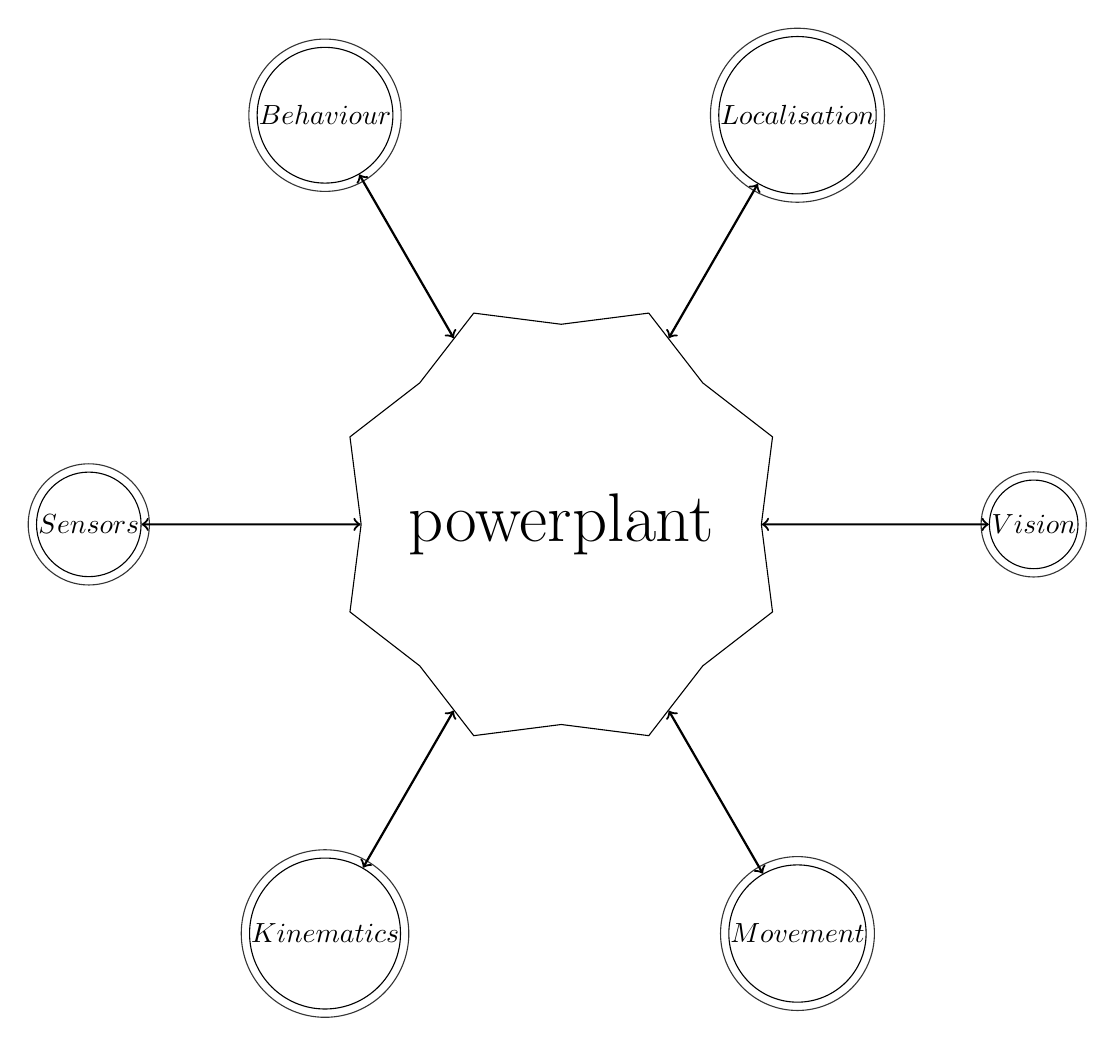
\begin{tikzpicture}

					% Draw our central Power Plant star
					\node [draw,star,star points=8,star point ratio=0.875,minimum width=5cm]
					(powerplant) {\Huge \gls{powerplant}};

					% Loop through each of our reactors
					\foreach [count=\i] \reactor in
					{Vision,Localisation,Behaviour,Sensors,Kinematics,Movement} {

						% Draw the reactors around the central star
						\node[draw,reactor] (reactorcircle) at ({360/6 * (\i - 1)}:6cm)
						{$\reactor$};

						% Draw a line from our reactor to our powerplant
						\path[readwrite] (reactorcircle) edge (powerplant);
					};
				\end{tikzpicture}
				\caption {The proposed architecture}
				\label{fig:HighLevelProposedArchitecture}
			\end{figure}

			The central authority of the proposed architecture is known as the \gls{powerplant} (Figure~\ref{fig:HighLevelProposedArchitecture} page~\pageref{fig:HighLevelProposedArchitecture}).
			The \gls{powerplant} is responsible for the primary communication functions of the architecture through a publish/subscribe message passing system.
			Only one \gls{powerplant} exists can per program and developers of the system are not likely to directly interact with it.

			The primary point of interaction for most users will be a \emph{\gls{reactor}}.
			When a user wants to create a new feature they create a new class that inherits from \gls{reactor}.
			This gives them access to the key functionality of the proposed architecture. This functionality revolves around two functions, \textbf{On} and \textbf{Emit}.

			\emph{On} allows users to specify \glspl{reaction} that behave as callbacks that are activated when new data is received.
			This is the method that is used to obtain data in a loosely coupled manner.
			The On method does not discriminate which component the data came from.
			This will be used by the robot in order to build on the results of previous components and perform logic.

			There are also a number of special types provided by the system.
			These types can be used in an \emph{On} statement in order to get different behaviour.
			The best example of this is the Every type. This type will make the system trigger the On method at regular intervals.
			This functionality will be used by the NUBots as the primal events that trigger all of the sensor reads each round.

			\emph{Emit} allows \glspl{reactor} to push data into the \gls{powerplant} that will then be distributed to all components that are interested in this datatype. This is done by calling their appropriate \emph{On} methods while providing the Emitted data as a parameter.
			This will be used by the robot to push the results of any operations it has performed to allow other components to use them.

			An example is that a sensor's reactor reads a camera frame every 30ms and uses \emph{Emit} to push a camera frame to the Power Plant. This is then received by the Vision system that processes the image and outputs the processed image it has created. This sequence of events is shown in Figure~\ref{fig:OnAndEmitExample} on page~\pageref{fig:OnAndEmitExample}.

			% On Emit and Every flow diagram
			\begin{figure}[h]
				\centering
				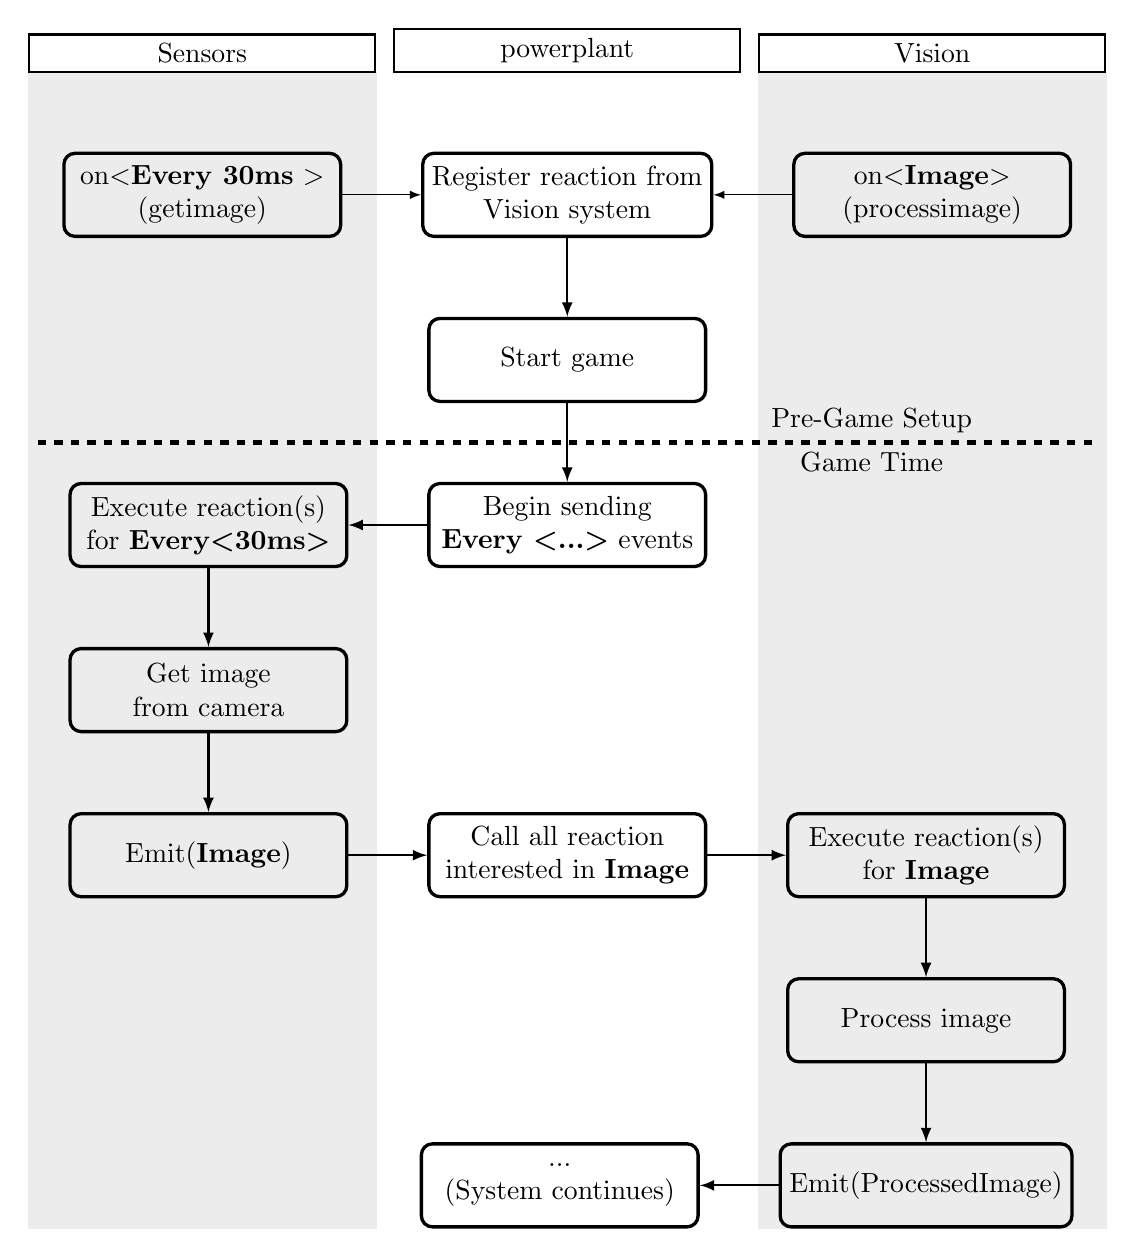
\begin{tikzpicture}[>=latex,
					block/.style={
						rectangle,
						rounded corners,
						draw=black, very thick,
						minimum height=3em,
						minimum width=10em,
						align=center
					},
					header/.style={
						rectangle,
						draw = black, thick,
						minimum height=1.2em,
						minimum width=12.5em,
						align=center
					},
					every join/.style={->, thick},
					chained/.style={every node/.style={on chain}}
				]
					\begin{scope}[start chain=going below, chained]

						% Draw the Register node and setup the following blocks to have arrows
						\node [block,join] (register) {Register \gls{reaction} from \\ Vision system};
						\begin{scope}[start branch=on going right, every join/.style={<-}]
							\node [block,join] (onimage) {on\textless \textbf{Image}\textgreater
							\\(processimage)};
						\end{scope}

						% Draw the on Every node
						\begin{scope}[start branch=on going left, every join/.style={<-}]
							\node [block,join] (onevery) {on\textless \textbf{Every 30ms}
							\textgreater\\(getimage)};
						\end{scope}

						% Start game node
						\node[block,join] (start) {Start game};

						% In Game every node
						\node [block, join] (runtimeStart) {Begin sending\\\textbf{Every
							\textless ...\textgreater} events};

						% Sensor Reactors node
						\node [block, join, on chain=going left] {Execute \gls{reaction}(s) \\for
							\textbf{Every\textless 30ms\textgreater}};

						% Get Camera Image Node
						\node [block, join] {Get image\\from camera};

						% Emit Node
						\node [block, join] {Emit(\textbf{Image})};

						% Image Call Node
						\node [block, join, on chain=going right] {Call all \glspl{reaction}\\interested
							in \textbf{Image}};

						% Execute Reactions Node
						\node [block, join, on chain=going right] {Execute \gls{reaction}(s)\\for
							\textbf{Image}};

						% Process Image Node
						\node [block, join] {Process image};

						% Emit Processed Image node
						\node [block, join] {Emit(ProcessedImage)};

						% Continuation Node
						\node [block, join, on chain=going left] (final) {...\\(System continues)};
					\end{scope}

					\coordinate (setuplineA) at ([xshift=-18em]$ (start) !.5! (runtimeStart) $);
					\coordinate (setuplineB) at ([xshift=18em]$ (start) !.5! (runtimeStart) $);
					\coordinate (setupTextPoint) at ([xshift=11em]$ (start) !.5! (runtimeStart) $);

					%% Setup dividing line and text
					\node [above] at (setupTextPoint) {Pre-Game Setup};
					\node [below] at (setupTextPoint) {Game Time};
					\draw [dashed, ultra thick, shorten >= -0.4cm, shorten <= -0.4cm]
						(setuplineA) -- (setuplineB);

					%% Add headers for the three threads
					\node [header,above=of onevery] (sensorsHeader) {Sensors};
					\node [header,above=of register] {\gls{powerplant}};
					\node [header,above=of onimage] (visionHeader) {Vision};

					%% Add the column backgrounds for Sensors and Vision
					\begin{scope}[on background layer]
						\filldraw [gray!15] (sensorsHeader.south west) rectangle
							(sensorsHeader.east |- final.south);
						\filldraw [gray!15] (visionHeader.south west) rectangle
							(visionHeader.east |- final.south);
					\end{scope}
				\end{tikzpicture}
				\caption {A flowchart example of how \textbf{On}, \textbf{Emit} and \textbf{Every}
					work}
				\label{fig:OnAndEmitExample}
			\end{figure}

			One of the key advantages of this design is that components are loosely coupled and only depend on the data format not changing.
			Therefore, the hardware dependent camera system could be replaced with a new module that reads from a prerecorded video stream for testing purposes.
			It also means that adding a new component to the system only requires the engineer to know what sort of data to access.
			As there is a single way to get data, there is no longer a need to track down an obscure method used to access the needed data.
			Instead, the engineer can tell the system the type required and the system locates it.

			Recent trends in computer hardware show that computational power increases come from increasing the number of cores available to the system.
			Unfortunately, the current system only takes advantage of, at most, two cores.
			The way that the system is currently architected enforces an artificial limitation on the resource utilisation of the system. Not making use of all the resources on the platform limits the potential of the final result.
			The proposed architecture takes care of multithreading transparently so the \gls{nubots} team can focus on figuring out the more important questions such as ``can this robot fetch me a pizza?''.
			When a \gls{reaction} is triggered, it does not always run immediately.
			Instead, the \gls{reaction} is put into a blocking priority queue and then executed on one of the many threads available to the \gls{powerplant} via a thread pool.
			For an example of how this system works see Figure~\ref{fig:PowerPlantThreadingOverviewDiagram} on page~\pageref{fig:PowerPlantThreadingOverviewDiagram}.

			% Power Plant Threading Diagram
			\begin{landscape}
			\begin{figure}[h]
				\centering
				\begin{tabular}{|l|l|l|l|}
					\hline
					Trigger                             & Task         & Emits            & Duration \\
					\hline
					\rowcolor{red!10}  Every 20ms       & Sensors      & SensorData       & 4ms \\
					\rowcolor{red!10}  SensorData       & Odometry     & OdometryData     & 3ms \\
					\rowcolor{red!10}  OdometryData     & Field Mapper & MapData          & 4ms \\
					\rowcolor{red!10}  MapData          & Map Combiner & Network\textless MapData\textgreater & 7ms \\
					\rowcolor{blue!10} Every 20ms       & Camera       & CameraImage      & 5ms \\
					\rowcolor{blue!10} CameraImage      & Vision       & ProcessedImage   & 7ms \\
					\rowcolor{blue!10} ProcessedImage   & Localisation & LocalizationData & 3ms \\
					\rowcolor{blue!10} LocalizationData & Behaviour    & MotorTask        & 2ms \\
					\rowcolor{blue!10} MotorTask        & Motors       & Nothing          & 2ms \\
					\hline
				\end{tabular}

				\vspace*{1 cm}

				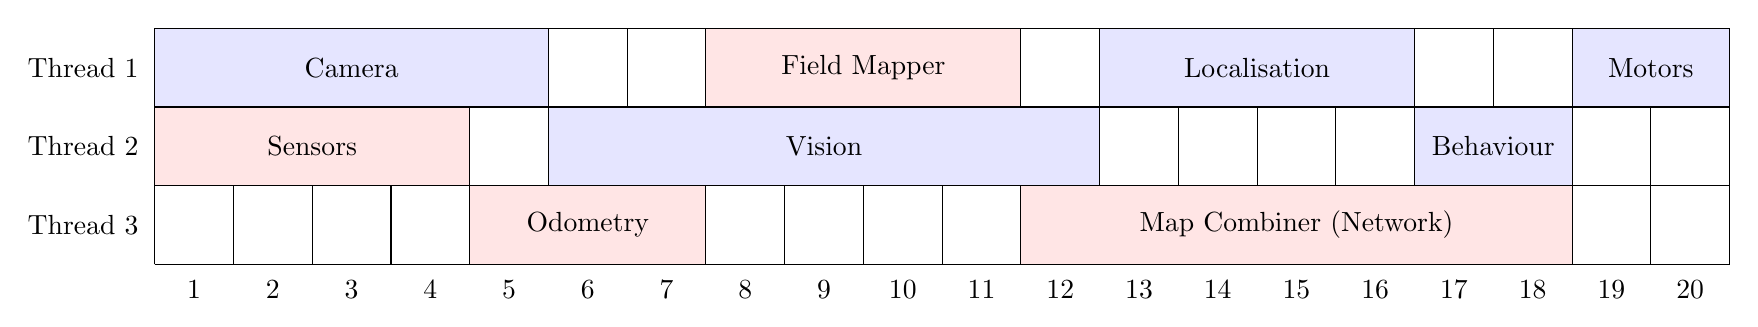
\begin{tikzpicture}

					\begin{scope}[
						task/.style={draw=black},
						cameratriggered/.style={fill=blue!10},
						sensortriggered/.style={fill=red!10}
					]

						\draw (1, 1) grid (21, 4);

						%% Thread 1
						\draw[cameratriggered, task] (1, 3) rectangle node {Camera} (6, 4);
						\draw[sensortriggered, task] (8, 3) rectangle node {Field Mapper} (12, 4);
						\draw[cameratriggered, task] (13, 3) rectangle node {Localisation} (17, 4);
						\draw[cameratriggered, task] (19, 3) rectangle node {Motors} (21, 4);

						%% Thread 2
						\draw[sensortriggered, task] (1, 2) rectangle node {Sensors} (5, 3);
						\draw[cameratriggered, task] (6, 2) rectangle node {Vision} (13, 3);
						\draw[cameratriggered, task] (17, 2) rectangle node {Behaviour} (19, 3);

						%% Thread 3
						\draw[sensortriggered, task] (5, 1) rectangle node {Odometry} (8, 2);
						\draw[sensortriggered, task] (12, 1) rectangle node {Map Combiner (Network)} (19, 2);

						% Row labels
						\node[anchor=east, inner sep=0] at (.8, 3.5) {Thread 1};
						\node[anchor=east, inner sep=0] at (.8, 2.5) {Thread 2};
						\node[anchor=east, inner sep=0] at (.8, 1.5) {Thread 3};

						% Column Labels
						\foreach \i in {1,...,20} {
							\node[anchor=north, inner sep=0] at (\i + .5, .8) {\i};
						}
					\end{scope}

				\end{tikzpicture}
				\caption {An overview of the \gls{powerplant} threading system}
				\label{fig:PowerPlantThreadingOverviewDiagram}
			\end{figure}
			\end{landscape}

			The client has also expressed how important it is that the robots be able to easily communicate. Networking is a difficult and error-prone process.
			It is imperative that the architecture provide a simple mechanism for robots to communicate.
			The proposed architecture allows an engineer to treat \glspl{reactor} on other robots as potential targets for the data.
			This means an engineer can emit data on one robot and receive it on any of the other robots. See Figure~\ref{fig:NetworkExampleDiagram} on page~\pageref{fig:NetworkExampleDiagram} for an example of how the networking system allows robots to cooperate and share data.

			% Networking diagram
			\begin{figure}[h]
				\centering
				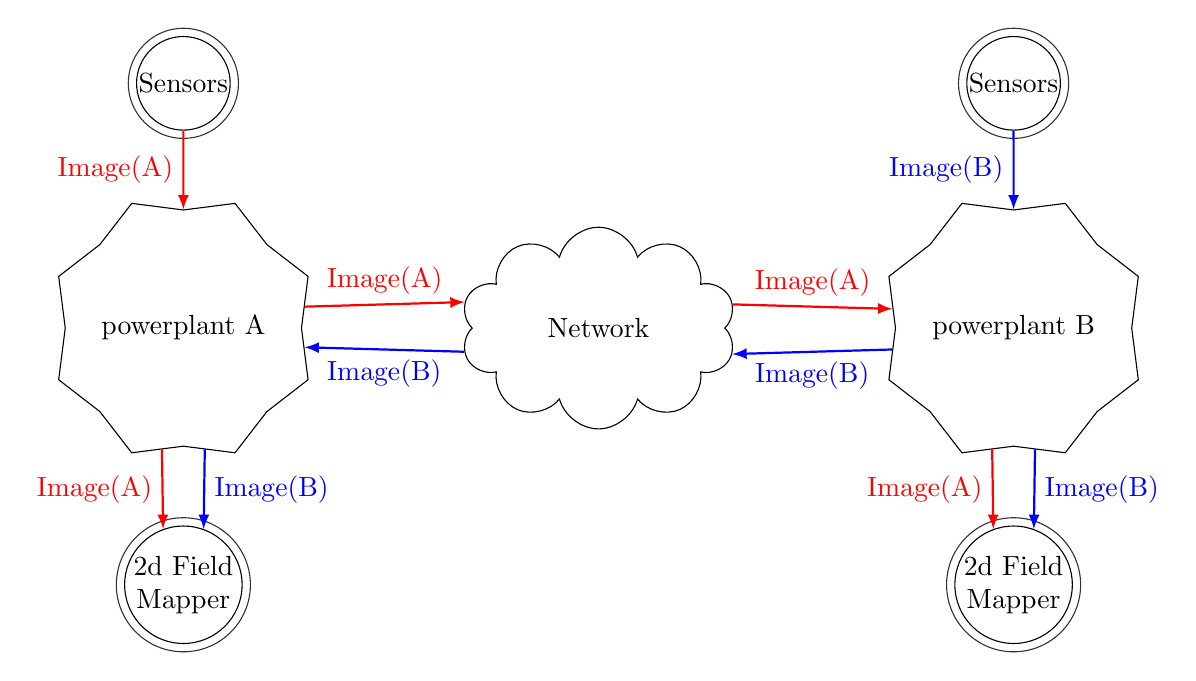
\begin{tikzpicture}[x=15em,y=5em,>=latex,
					A/.style={red},
					B/.style={blue}]

					%%% Left Power Plant
					\node at (0, 0)
						[draw,star,star points=8,star point ratio=0.875,minimum width=3cm]
						(plantA) {\gls{powerplant} A};
					\node [above=of plantA,reactor] (sensorsA) {Sensors};
					\node [below=of plantA,reactor,align=center] (fieldmapperA) {2d Field\\Mapper};
					\path [A, write] (sensorsA) edge node[A,left] {Image(A)} (plantA);
					\path [A, read] (fieldmapperA.110) edge node[left] {Image(A)} (plantA.260);
					\path [B, read] (fieldmapperA.70) edge node[right] {Image(B)} (plantA.280);

					%%% Right Power Plant
					\node at (2, 0)
						[draw,star,star points=8,star point ratio=0.875,minimum width=3cm]
						(plantB){\gls{powerplant} B};
					\node [above=of plantB,reactor] (sensorsB) {Sensors};
					\node [below=of plantB,reactor,align=center] (fieldmapperB) {2d Field\\Mapper};
					\path [B, write] (sensorsB) edge node[left] {Image(B)} (plantB);
					\path [A, read] (fieldmapperB.110) edge node[left] {Image(A)} (plantB.260);
					\path [B, read] (fieldmapperB.70) edge node[right] {Image(B)} (plantB.280);

					%%% Network & Network Connections
					\node at (1, 0) [draw,cloud,cloud puffs=10,minimum width=3.5cm]
					(network) {Network};

					%% Plant A connections
					\path [A, write] (plantA.10) edge node[A, above] {Image(A)} (network.169);
					\path [B, read] (plantA.-9) edge node[B, below] {Image(B)} (network.190);

					%% Plant B connections
					\path [A, read] (plantB.171) edge node[A, above] {Image(A)}  (network.10);
					\path [B, write] (plantB.190) edge node[B, below] {Image(B)} (network.-11);

				\end{tikzpicture}
				\caption {An example of how robots can communicate camera data over a network to
					build a 2d map of the field}
					\label{fig:NetworkExampleDiagram}
			\end{figure}

	\section{Non-Goals}
		This section addresses areas of the system that are out-of-scope for the proposed architecture.
		The proposed architecture will make no effort to address these issues directly, however, some out-of-scope components will benefit indirectly from improved architectural consistency.

		\subsection{Algorithm Changes}
			The \gls{nubots} system contains a number of complicated mathematical systems that are used by the robot to analyse the world, make decisions and control its interactions within its environment.
			The proposed architecture will not change these algorithms beyond any necessary changes required to integrate them into the new architectural style.
			However, the method by which an algorithm gets its inputs may be modified, but the mathematical algorithm it is based on will not be modified.

		\subsection{Hardware Changes}
			The proposed architecture is targeting an abstract computing platform with no specific hardware available to be identified.
			However, the components of the existing system that are to be ported over, are currently based on the \emph{DARwIn-OP} platform.
			This assumes that there is some form of networking and processing.
			However, the project team will impose no requirements on the existing or future hardware.
			Furthermore, the proposed architecture will not require any changes to the robotic hardware in order to run.

	\section{Scenarios}
		This section covers some common scenarios in robotics programming and how they would be resolved
		using both the existing and proposed architecture.

		\subsection{New Functionality Added to System}
			The robot currently consists of several integrated components allowing it to play soccer.
			However, to enhance its ability to play effectively, new components may be added to the system.
			These components will either augment existing abilities or provide new functionality.

			\paragraph{Scenario} Due to a recent rule changes in the
			\emph{\gls{robocup} humanoid division}, the goal posts are no longer different colours.
			Therefore, a new component must be added to the robot's software allowing it to determine the direction it is facing.
			In the event that the robot falls over this component would break the field symmetry and reorient the robot.
			The component responsible for finding the direction would require access to existing sensor input and its output would need to influence the localisation system.
			The team has already developed a system that is able to determine the direction the robot is facing by looking at features above it.
			The team will integrate this system with the current codebase.

			\subsubsection{Current System}
				In order to implement this in the proposed system, the following changes are required:

				\begin{itemize}
					\item Vision would need to be modified in order to allow the compass to use the image frame.
					\item The compass code would need to be inserted into the global program flow following the current vision system so required image exists, but before localisation.
					\item Behaviour would need to be modified to instruct the robot to look up.
					\item The Job system would require a new Job class to be created and new code written in order to route this correctly.
					\item Blackboard would need to be modified in order to provide a new location for the output of the Compass.
					\item Localisation needs to be modified to read this information and apply it to the robots localisation.
				\end{itemize}

				It is important to note that as vision is the only system that is set up to obtain images from the \emph{SenseMove} thread, the vision system would need to be modified to allow for multiple systems accessing the camera images.
				This would require putting in safeguards to prevent the vision from modifying the image on the blackboard and doing the same in the new compass system, to ensure that they did not influence each other’s results.
				As a result of the new compass system, it becomes less clear which component is responsible for requesting the new vision frame from sense/move.
				If these two systems run on alternating frames, the system that requests the new frame must be carefully selected.

				In order to integrate the compass the user needs an understanding of the following systems interactions \emph{Vision}, \emph{Behaviour}, \emph{Job System}, \emph{Blackboard} and\emph{Localization} as well as the global program flow in order to ensure that the correct system requests a vision frame.

			\subsubsection{Proposed System}
				In order to implement this in the proposed system, the following changes would be required:
				\begin{itemize}
					\item The compass code would need to be set up to use images as they arrive and emit its direction to the power plant.
					\item Behaviour would need to be modified to instruct the robot to look up.
					\item Localisation would need to be modified to utilise the new Compass information.
				\end{itemize}

				In order to integrate the compass the user needs an understanding of the following systems interactions \emph{Behaviour}, \emph{\glspl{reactor}} and\emph{Localization}

				There are fewer systems that are affected by this change in the new architecture, and the consistent method of communication between them means that there is no longer a need to understand both blackboard and the job system.
				The method by which messages are passed also means that no global state needs to be set up to hold the new information provided by the compass.

			\paragraph{Scenario} The marketing department for Engineering wishes to use the NUBots robots for advertising purposes. They request that the robots be made to dance in time to music they plan to play through speakers. Therefore a new component will need to be added to take audio input and analyse it to determine how the robot should dance. Dance move scripts will need to be added to the system and a way to execute the scripts according to timing of the beats.

			\subsubsection{Current System}
				In order to implement this in the current system, the following changes would be required
				\begin{itemize}
					\item An audio input component would need to be added to take in audio through the microphone that is currently unused.
					\item An audio processing component would need to be added to analyse the audio to determine how it should dance.
					\item The script system would need to modified to include many dance scripts.
					\item The Behaviour system would need to be modified to allow the dance scripts to be executed in time to the beat of the music that was detected.
					\item Blackboard would need to be modified in order to provide a new location for the output of the audio processing.
				\end{itemize}

			\subsubsection{Proposed System}
				In order to implement this in the proposed system, the following changes would be required:
				\begin{itemize}
					\item The script system would need to modified to include many dance scripts.
					\item The Behaviour system would need to be modified to allow the dance scripts to be executed in time to the beat of the music that was detected.
					\item An audio input component would need to be added to take in audio through the microphone that is currently unused.
					\item An audio processing component would need to be added to analyse the audio to determine how it should dance.
				\end{itemize}

		\subsection{Networking with other Robots}
			Many modules within the robot’s code can benefit from information gathered by other robots on its team.
			Sharing information, such as the position of objects on the field and each robot’s current action, allows better co-operation.
			Another advantage provided by networking is the opportunity for distributed computing on computationally or spatially intensive problems.

			\paragraph{Scenario} The \emph{\gls{nubots}} team have decided to improve their behaviour system to promote better teamwork between the robots.
			To facilitate this, the robots need an easy method to communicate their intentions to each other across the network.
			The networking system needs to serialise the data from the behaviour system and deserialise this data on the receiving robots.

			\subsubsection{Current System}
				The current system does have a networking solution, however, it is modified on a case by case basis to provide network traffic.
				In order to implement this, the following changes would be required:
				\begin{itemize}
					\item Behaviour would need to be modified to output its state.
					\item A serialisation/deserialization method for the state would need to be written.
					\item A new networking component for behaviour would need to be integrated with the existing network stack
					\item Behaviour would need to be modified to search the incoming network traffic queue to find behaviour packets.
					\item Behaviour would need to be modified to take advantage of information from other robots.
				\end{itemize}

				The current system performs networking at the socket level.
				This means each component that wants to communicate over the network must interact directly with the operating system.
				Adding any communication between the robots requires an understanding of both Windows and Linux style sockets.
				An understanding of how the existing network traffic is sent is required so that all components send information over the same port.
				This means that when the behaviour system needs to read the new relevant information, it must read through all the incoming traffic to find behaviour data.

			\subsubsection{Proposed System}
				The proposed architecture provides networking as part of the standard \gls{powerplant} interface.
				In order to implement this in the proposed modification, the following changes would be required:
				\begin{itemize}
					\item Behaviour would need to be modified to output its state
					\item Behaviour would need to be modified to take advantage of information from other robots.
				\end{itemize}

				The number of changes required in the scenario with the proposed architecture are substantially reduced.
				This is because the proposed architecture provides an abstraction over networking that simplifies the use of networked logic.
				As this abstraction is built into the architecture, there is no additional effort required between sending packets between robots and using local information.

		\subsection{Moving to a new hardware platform}
			Currently there are many robotic platforms that are available for the development of autonomous
			robotic systems. In previous years the \emph{\gls{nubots}} team have made use of the \emph{Sony AIBO},
			the \emph{Aldebaran Nao} and the \emph{Robotis DARwIn-OP} platforms. Additional robotic platforms will be used as technology progresses, requiring that the code be ported to the new platform.
			Ideally this action will result in a minimal number of changes to the code base.

			\paragraph{Scenario} After a number of years, the Darwin-OP platform has become obsolete and a new platform, the Super Turbotron 5000, has been selected as its replacement. It has twenty
			additional degrees of freedom, stereo vision and two giant laser cannons. The system must be
			adapted to be able to utilise these changes with a minimal amount of impact to the existing codebase, as well as be able to still operate on the Darwin-OP during the transition.

			\subsubsection{Current System}
				The current system handles platform changes through a series of conditional compilation flags throughout their source files.
				There are more then ten different components that rely on compiler flags to determine what platform they are targeting.
				This is a complex change that affects the majority of the system and requires someone who understands the entire system.

				New components would need to be written to replace all of the hardware dependent components. This includes reading sensors, moving motors, kinematics and any other components that incidentally communicates to the robot's hardware.
				Additionally all the systems that communicate to the affected components may also need to be modified.
				Typically this cascades to a system-wide modification.

			\subsubsection{Proposed System}
				Because of the loose coupling between components, it is likely that it will only be necessary to replace the components that directly depend on the robot’s hardware.
				All low-level conditional compilation is rendered obsolete in the proposed architecture with only a skeleton remaining to tell the system which high-level components to activate.

				The majority of the system would remain unchanged. New components for hardware would still need to be written and old components may need to be updated to take advantage of new hardware.

				However the \gls{powerplant} itself is not a safeguard against this form of change. If the new system was used in such a way where low level hardware decisions were made in areas such as behaviour, rather then restricting this logic to motion, then the new architecture will not provide a significant benefit over the existing system.

		\subsection{Debugging bad Data}
			\begin{quote}``Debugging is twice as hard as writing the code in the first place. Therefore, if you write the code as cleverly as possible, you are, by definition, not smart enough to debug it.'' - Brian Kernighan\end{quote}
			One of the most useful techniques available for software debugging is being able read inputs and outputs for a section of code. Once the data that enters a section
			of code is known, the remainder of the code can be analysed by hand to ensure that each
			step has the expected result. Tracing the data through the system to where the unexpected results start reveals the source of the problem.

			\paragraph{Scenario} The \gls{nubots} team have encountered a problem where the robot after
			receiving a notification that it kicked an own goal, will proceed to breakdance instead
			of hanging its head in shame. They have identified that this activity is due to the
			\em{Breakdance} action being performed instead of the expected \em{SadRobot} action. However, they are unable to identify why this action is being performed and need to trace the source
			of this logical error.

			\subsubsection{Current System}
				In the existing system, tracing is done through manually adding print statements to the code in the affected areas.
				Some systems have the ability to write their data to the network to be viewed in real time, but this is provided on a per-component basis and the exact mechanism differs for each component.

				For this particular problem, trace statements need to be added to the Behaviour, Motion and Job systems to determine why this particular job is called and why the robot is kicking its own goal in the first place.
				After these statements are added, the \gls{nubots} team then need to identify the issue through the trace logs, write a fix and then run it live on the robot. If the fix fails then the process must be repeated until the bug is fixed.

			\subsubsection{Proposed System}
				In addition to standard logging capabilities, the proposed architecture also provides the ability to capture the entire input sequence for a particular component.
				This means the exact inputs can be captured that caused the robot to kick an own goal and then breakdance.
				Once the inputs have been captured, they can be turned into a unit test that, in many cases, can be run independently from the robot.

				Once the system has provided a unit test, all that remains is to write a fix.
				However, in many cases, this fix may be tested on the development machine instead of the robot.
				If the unit test passes, then the code can be deployed to the robot and tested to find if the problem is solved.
				This greatly reduces development time, as testing on the robot hardware is time consuming and intermittent.
				This approach also has the benefit of slowly building up a library of unit and regression tests against known bugs.

		\subsection{The Robot is used to perform a new task}
			Robotics is an expanding field of research with robots being applied to an increasing number of tasks.
			Each of these tasks are often performed on the same robotic platforms and need to perform similar tasks.
			This provides a huge opportunity for code reuse among these tasks.
			However, code that is difficult to understand, or separate from the surrounding code, may be ignored in favour of rewriting the required functionality.

			The \gls{nubots} team have been asked to add dancing capabilities to the robot to help market the university.
			The university wants the robot to be able to dance to a beat and compete in ``So you think you can RoboDance''.
			The \gls{nubots} team realises that some of their existing code can be leveraged to build the dance subsystem.

			\subsubsection{Current System}
				In the existing architecture reuse of code is primarily achieved by copy and paste.
				This is especially evident in places where there are multiple implementations of the same concept.

				Allowing the robot to dance requires a new behaviour module that contains the dance state machine.
				Additionally, the sensor system will need to be modified to provide sound information to the new dance component.

				The kinematics model in the existing system is also very useful for dancing.
				Unfortunately, access to the kinematics model is very difficult in the current system and requires a lot of hoop jumping to gain access to the appropriate data.

				Both the blackboard and jobs systems need to be modified to accommodate the new data.
				The two main threads will need to be modified to change from ``play soccer'' to ``dance''.
				This involves an error prone process that requires unlinking all non-dance related methods from the loop.

			\subsubsection{Proposed System}
				In the proposed architecture, reuse of code is achieved by adding/removing modular \glspl{reactor} that communicate through the \gls{powerplant}.
				Firstly, a new sound \gls{reactor} that buffers sound input and emits it periodically would be created.
				Then a sound analysis \gls{reactor} that determines the beat and emits the ``feel of the song'' should be created.
				A modified behaviour \gls{reactor} would react to the beat of the song and perform the dance.

				Once the components are created, the engineer needs to tell the \gls{powerplant} to use them.
				The old soccer-based behaviour from the system needs to be removed, but unlike the existing architecture, this is a simple one-line change per component.

	\section{Requirements}
	This requirement section considers the requirements for the NUClear architecture framework and the task of the robot dance that will use NUClear.

		\subsection{NUClear Requirements}
			The requirements defined in this section are used to provide a set of measurables to determine if the final architecture achieves its goals.
			It also provides a baseline to compare this architecture against both the architecture it is replacing as well as other competing architectures.

			\subsubsection{Multiprocessing}
				\requirement{The architecture must take advantage of all CPU cores}

				The existing system is currently only able to take advantage of two cores.
				Unfortunately, writing multithreaded code is difficult and distracts programmers from more important things such as improving the speed at which a robot can backflip by 5\%.
				To account for this, the proposed API must provide a way for programmers to easily utilise the full CPU power of any robot platform.

				This requirement is becoming increasingly important.
				The current trend in computing performance is to add more cores, so it is important that all resources are utilised.

				From an API point of view, the ideal acceptance test for this requirement is to determine how often a programmer needs to think about multithreading at all.
				The project team could analyse the code to determine what sections need to include multithreaded primitives and from that percentage determine how many times the API failed to provide the proper multithreaded abstractions.
				However, from a performance and hardware point of view, the project team can measure CPU utilisation on various platforms and compare it to the old system.

				From a performance and hardware point of view we can measure CPU utilisation on various
				platforms and compare it to the old system.

				Technical Note: The project team is assuming that limited single-core machines will be used.
				The API should still support single threaded machine.

			\subsubsection{Robot Platforms}
				\requirement{The architecture must be portable to new platforms}

				The existing system contains complicated logic that is used to support a few different platforms.
				It is currently not possible to easily swap out the Darwin motor components for an \emph{AIBO} or \emph{Nao} motor component due to the tight coupling of systems.

				The new architecture should provide a way to easily slot in platform dependent components.
				For example, it should be possible to remove the hardware-dependent Darwin camera component and replace it with an AIBO component with minimal to no modification of other components.

				Portability can be measured by determining the amount of code that depends on specific hardware or platforms.
				For this exercise, Unit Tests can be considered another platform to determine the portability by replacing hardware-dependent components with mock components.

				Technical Note: If the format of the data changes, the systems that rely on that data need to change as well.
				The project team aim to reduce unnecessary changes due to API bloat.

			\subsubsection{Performance}
				\requirement{The architecture must have acceptable performance}

				Robotic platforms have strict requirements about how often motors need to be sent commands.
				If these performance requirements are not met, the robot’s usefulness is limited.
				These requirements limit the processing or resource costs to the existing system.

				A good example of a system that imposes heavy performance costs is Robot Operating System (ROS).
				ROS has made a number of trade-offs to facilitate distributed multi-language multi-platform systems, but those trade-offs have resulted in unacceptable performance implications for smaller robots such as the Darwin.

				The proposed architecture should be optimised to run efficiently so it does not take valuable resources away from critical computations.
				Ideally, the architecture should be structured in a way that it can assist the \gls{nubots} team in writing efficient code.
				The first key indicator of performance is to determine the ratio of time used by the architecture vs. the time taken by actual components.
				The ratio should be so small as to be practically insignificant. A good architecture should also provide the tools to measure performance.

				The speed of the old architecture vs. the new architecture can also be measured to determine what improvements have been made.

			\subsubsection{Component Interfaces}
				\requirement{The architecture must promote consistent interfaces between components}

				In the existing system there are a number of ways components can communicate.
				A significant limitation is that it greatly increases the complexity of the system and also causes increased coupling due to all the different ways components can communicate.

				The proposed system needs to provide a unified mechanism for components to communicate.
				However, this unified mechanism should not require the removal of any existing functionality and must be able to accommodate or replace any of the existing communication styles.
				By providing a unified mechanism, the complexity of the system can be reduced.

				This requirement can be measured by analysing the mechanisms that components use to communicate.
				For example, the places the Camera system communicates with the Vision system can be examined to determine the number of unique ways in which they communicate.
				Additionally, the suitability of the unified mechanism can be measured by ensuring that it does not require removal of any existing functionality.

			\subsubsection{Adding Components}
				\requirement{The architecture must make it easy to add new components to the system}

				Adding a new component to the existing system is comparatively difficult.
				This is because it currently requires a broad knowledge of existing systems due to their tight independence.
				Because the existing communication methods through blackboard are tightly coupled, adding a new component may cause unintended side effects in other modules.

				This is one of the key components the new architecture needs to solve.
				Ideally, any new component should only require knowledge of the inputs and outputs of that component.
				The proposed architecture must provide a mechanism to simplify adding new components to the system.

				This requirement is best measured by comparison against the old system.
				For example, a new behaviour could be added to the system to handle catering at university functions.
				It could then be analysed how many components would need to be understood and changed to add this new component. A metric could be developed to analyse the extent of the changes.

			\subsubsection{Networking}
				\requirement{The architecture must provide methods to easily perform network
				communication}

				Communication is a vital part of any team activity, without communication there is no way to work on team behaviour, or share useful information.
				The current system has a limited networking solution.
				It is difficult to use, which deters coders from using it to better the team abilities of the robots.
				By providing a simple and intuitive interface to send and receive networked data, a greater range of possibilities of team behaviour and distributed computing becomes accessible to the \gls{nubots} team.

				The new architecture must be able to automatically find and communicate with any robots that are currently on the network without configuration (auto discovery).
				It also must be able to serialise packets of data into a binary format for the majority of cases, and allow the user to provide a serialiser for any edge cases.
				The cases that should be covered by the system and as a minimum, any data type that contains only Plain Old Data (a container of basic data types only), or an instance of a Google Protocol Buffer.

				This requirement is measured by the amount of code that is required to both send and receive network packets from other robots, as well as how efficient the binary representation over the network is.
				For example, take the case of the two robots bragging about how they went after the game.
				Being robots, it would be inefficient to communicate using a natural language such as English, they would not be able to convey their level of awesome quickly enough (running out of bandwidth).
				As such, all information exchanged should be in a binary format.
				Also, as the robot is made up of many individual components, the communication between these components, must use the same communication channel, but have different origin and destination points.

			\subsubsection{Debugging Tools}
				\requirement{The architecture must provide tools for debugging components}

				Debugging in the current system is a very difficult and painful process. Since all of
				the components are so tightly integrated with each other, this means that if an error
				occurs in one system, it is difficult to locate where the source of the error was. For
				example, in the current system an issue exists where if the camera is not connected, the
				vision system (the next system in the pipeline) will progress to the point of
				classifying the image before the robot crashes. This makes it appear that the bug is
				located in the vision system, however, it is actually located in the camera reading
				system.

				The new architecture should provide tools within it that allow the debugging of both
				errors with the systems, as well as the performance between the systems. Using the tree
				style model of communication between components, it is possible to output this tree into
				a format that is understandable. This would allow the person debugging the system to see
				where each data packet that was used in the system of interest came from, and if enabled
				the contents of those data packets should also be available in order to replay the
				scenario that caused the error.

				These debugging tools can be measured by comparing the difficulty of tracing data through a system. It can also be measured by the ability to easily replay the data through the system to see the results.

			\subsubsection{Testing}
				\requirement{The architecture must provide tools for unit testing individual components}

				Unit testing is a very important concept as it allows a number of tests to be performed
				on individual components in the system. This can help to identify and kill bugs before
				they even leave the development environment. By enforcing greater isolation between the
				components, the architecture is able to make it much easier to test an individual
				component by sending it fake data and validating the results.

				The system must provide a testing harness that makes it easy to test in isolation a
				component of the system. This testing harness should be able to wrap around any of the
				individual components that make up the system and, without modification to the component
				itself, send fake input to the component and capture and validate any output from that
				system. This should allow the system to be unit tested thoroughly so that the number
				of bugs that exist when the code is executed on the robot is much lower.

				This requirement is measured by comparing the difficulty of testing a component between
				the current system and the new system. This includes both the difficulty of extracting
				the component from the system to be tested without other components (isolating the
				component) as well as the difficulty of testing its API and results once it has been
				extracted from the system.
		\subsection{Dance Requirements}
		This section deals with the requirements of making the robot dance.
			\subsubsection{Dancing to a script}
				\requirement{The robot must be able to dance by executing a script}

				A script will specify what actions the dance move consists of.
				This script will be run by the kinematics module. Running scripted dance is a necessary requirement.
				It will need to be able to run the dance scripts directly and also run them based on music that is being played or in response to movements detected by the camera.
				The scripts do not need to involve leg movement, but only arm movement.
				The scripts need to be written so that they cannot cause the robot to fall over or damage itself.

				Testing will be done by observing whether the robot can carry out the dance moves as expected.
				It will also involve testing on a more technical level to see what reasons the moves may be aborted, for example, not enough room to perform move or whether the robot has fallen over.

			\subsubsection{Audio Input}
				\requirement{The robot must be able to take audio input through it's microphone}

				The robot will several times a second record a short snippet of sound.
				This is to record the sound to a similar quality to what a human would be hearing in the robot’s position.
				In the music analyser stage, the last several snippets of recordings will be combined, ready for analysis.
				The recording must use the Darwin robot’s microphone. This feature is necessary for the requirement of dancing according to music.

				A testing module will be created that converts the recording to a sound file to be checked for quality by a human.
				For testing, the length of the recording snippet will be increased to a length significantly long enough for a human to be able to hear it properly.
				Only the human ear will be able to tell whether the sound was recorded in a way that is faithful to the sound the audience would be hearing.

			\subsubsection{Dancing to Music}
				\requirement{The robot must be able to dance according to the beat of the music detected through it's microphone}

				The location and frequency of the beat will be detected. Beat is the basic timing element of music.
				A person tapping their foot to music is detecting the beat and following it.
				Any piece of music with a beat should be able to be analysed to find the beat.
				From simple clapping to a piece of classical music, the beat should be detected.
				The beat of the analysed music must be compared with the possible dance moves that will specify what range of beats the dance move is capable of working for.
				One of the valid dance moves will be chosen and the dance script will be scaled in time to fit the beat.
				The robot must not repeat the same dance moves again and again if possible, but will alternate between different dance moves.
				The beat tracker must be able to tell when one musical item ends and another starts. It must ignore the first musical item, and only calculate the beat on the audio of the second musical item.
				The beat tracker is not expected to be able to detect the beat on complicated music, such as music without drums.
				The beat tracker must be able to detect the beats on audio that has background noise, including people talking and fan noise from the robot’s motor.
				It is not expected to be able to find the correct beat if the background noise includes other music. The beat tracker must emit the location of the beat within 50ms after the beat has occurred.

				Beat tracking will be tested by running the beat tracking algorithm on a large sample of music.
				The results of this will be recorded. The results will then be compared to the actual beat locations of the music using a suite of evaluation algorithms.
				These evaluation algorithms will be those used in the beat tracking research community based around the Music Information Retrieval Evaluation eXchange (MIREX).
				The scaling of dance moves according to beat will be tested by flashing the robot’s eyes according to the beat to show its response to the beat.

			\subsubsection{Demonstrate the NUClear Architecture}
				\requirement{The robot dance will demonstrate the qualities of the NUClear architecure}

				The dance part of the project is mainly to demonstrate the success of the NUClear architecture. It will show that the NUClear architecture:
				\begin{itemize}
					\item{Allows systems to be easily extended}
					\item{Allow systems to be easily adapted for other purposes}
					\item{Allow easy component re-use}
				\end{itemize}

				This requirement will be measured by the number of components changed to add new functionality, compared to the estimated number of components needed to be changed under the old system.

	\section{Extension Goals}
		This section will outline extra goals that are not requirements, but would be useful to have with additional time.
		None of these should be implemented before a requirement unless the requirement implementation trivially adds an extension.

		\subsection{The architecture could support ROS (Robot Operating System) integration}
			The proposed architecture could provide systems to make ROS component integration easy.
			Currently, the existing system does not contain any facilities for ROS integration.

			Additionally, no other \gls{robocup} teams have any degree of ROS support.
			Having ROS support would provide a competitive advantage.
			This goal can be measured by checking the integration of a ROS component.

	\printglossaries
\end{document}
